\documentclass{amia}
\usepackage{graphicx}
\usepackage[labelfont=bf]{caption}
\usepackage[superscript,nomove]{cite}
\usepackage{color}
\usepackage{multirow}


\begin{document}


\title{Comparison of clinical trial with the results obtained from EHRs along with missing value analysis}

\author{Mehedi Hasan, BS$^{1}$, Alexander Kotov, PhD$^{1}$, Rick Krajenta, BS$^{2}$, Melody J. Eide, MD, MPH$^{2,3}$, Christine C. Johnson, PhD, MPH$^{4}$}

\institutes{
$^1$Department of Computer Science, Wayne State University, Detroit, Michigan; 
$^2$Departments of Biostatistics and Research Epidemiology,
$^3$Department of Dermatology, 
$^4$Department of Public Health Science, Henry Ford Health System, Detroit, Michigan\\
}

\maketitle

\noindent{\bf Abstract}
\textit{This study compared the PLCO survey response with the results obtained from electronic health records. Our study also explored the missing data problem and offer advice for dealing with missing data. To extract clinical information, we built an integrated information extraction system that leveraged several publicly available clinical NLP and information extraction tools. Experimental results showed the significant difference between these two results, while extraction results achieved 91.2\% to 100\% accuracy. The structure of missing values was analyzed with visualization tools implemented in R-package. We observed MAR situation for certain variables such as ``quit time'', ``smoking duration'', and ``pack-year smoked''. These results indicate that EHR data contained sufficient information can be used directly for certain research. Besides that, a clinical trial might be suffered by missing values or biasing or noise occurred during the trials. These problems can be resolved with EHRs in combination with properly addressing missing values.}


\section*{Introduction}
Electronic health records (EHRs) are increasingly being used to document and store large amounts of clinical information \cite{jha2009use}. They replaced traditional paper-based systems in many healthcare organizations and became a vast data sources which can facilitate clinical research and studies to ultimately improve healthcare quality \cite{blumenthal2010launching, erickstad2011use, lau2011use}. Much of the available clinical data are in narrative form as a result of transcription of dictations, direct entry by providers, or use of speech recognition applications. Comparing to structured data, free text is a more conventional way in the health care environment to express concepts and events. However, free text is very challenging for searching, summarization, decision-support, or statistical analysis. To reduce medical errors, improve health care quality, and enable secondary use of EHRs, information extraction (IE), which structures and encodes clinical information stored in free text, is necessary. However, traditional natural language processing (NLP) tools are not designed for the fragmented free text found in narrative clinical records; therefore, they do not perform well on this type of data. 

In the past decade, several different techniques have been developed to extract information, from simple pattern matching to complete processing methods based on symbolic information and rules or based on statistical methods and machine learning. Many prior natural language processing (NLP) studies in the clinical domain have used regular expressions in designing their NLP solutions \cite{stenner2012paste,piwowar2008identifying,denny2009identifying, mccart2012using,xu2011facilitating,matheny2009detection,zeng2006extracting,huang2007novel}. These regular expressions are typically created by software developers working with domain experts. One of the important regular expression based work is NegEx \cite{chapman2001simple}. This is because significant portion of medical text is negated in electronic health records. NegEx depends on a list of phrases that indicate the absence of a particular medical condition such as disease or symptom to negate the conditions within a window of five words or phrases. 

An extended version of NegEx called ConText \cite{harkema2009context} was proposed to determine three contextual features including negation (negated, affirmed), temporality (historical, recent, hypothetical) and experiencer (patient, other). To encode these contextual features, several NLP systems have also been designed to encode detailed information from clinical reports, such as MedLEE \cite{friedman2000broad}, MPLUS \cite{christensen2002mplus}, and MedSyndikate \cite{hahn2002medsyndikate}.

However, health information text extraction (HITEx \cite{zeng2006extracting}) was developed to extract diagnoses and smoking status. Statistics shows that smoking causes nearly one of every five deaths in the United States each year. Therefore, extraction of patients smoking status is necessary for clinician and researcher. Mayo Clinic developed an NLP System named clinical text analysis and knowledge extraction system (cTAKES \cite{savova2010mayo}) to extract clinical information from medical domain. Additional modules have been implemented within cTAKES recently \cite{savova2008mayo} for identification of patient smoking status.   
 
While substantial progress has been made in the development of NLP tools, no information extraction (IE) system is perfect for extracting all kind of variables in different domain, and still suffer from various weaknesses. In this study, we built an integrated system that leveraged several existing NLP components. Experimental results shows that our system performed well in biomedical domain. 

In this study, we mainly focus on findings from electronic health records and then compare the result with PLCO clinical trial. We also describe missing patterns observed in our experiment. This paper reports that which information are sufficiently available in EHRs for conducting clinical research. It also states that which of the variables are noisy in clinical trials. These findings are significant in clinician and researcher who are conducting their research with clinical trials or EHRs. To the best of our knowledge, there is no report that compare the results between response from clinical trials and NLP-based extraction from EHRs. 

\section*{Methods}
\subsection*{\textit{Data collection}}
Four hundred and fifty thousand free-text EHRs of 11,968 patients were obtained from Henry Ford Health System, who participated in the PLCO clinical trial. Out of this 11,968 patients, 1000 patients were randomly selected for this study. The PLCO trial began enrolling participants in November 1993 and completed recruitment of 154,938 subjects over different health systems in June 2001. Men and women aged from 55 to 74 years participated in the PLCO trial at ten screening centers nationwide with balanced randomization to intervention and control arms. All participants received a posterior anterior view chest x-ray for lung cancer screening. A baseline epidemiological questionnaire and a supplemental questionnaire (SQ) were administered as part of the PLCO surveys. The obtained patient EHRs consist of different types of clinical documents including clinical practice guidelines, diagnostic reports and discharge summaries.

\subsection*{\textit{System overview}}
We built an integrated information extraction system that leveraged several publicly available clinical NLP and information extraction tools. In particular, our system consists of the following components: 1) A sentence boundary detection program, which was developed at OpenNLP \cite{morton2005opennlp}; 2) an existing corpus based section identification program (SecTag \cite{denny2009evaluation}); 3) regular expression based NLP program that utilizes the clinical Text Analysis and Knowledge Extraction System (cTAKES \cite{savova2010mayo}) and contextual feature extraction system (ConText \cite{harkema2009context}); 4) post processing program that maps our results into PLCO compareable format. Figure \ref{fig:extraction} shows the architecture of our system. 

\begin{figure}[h!]
\centering
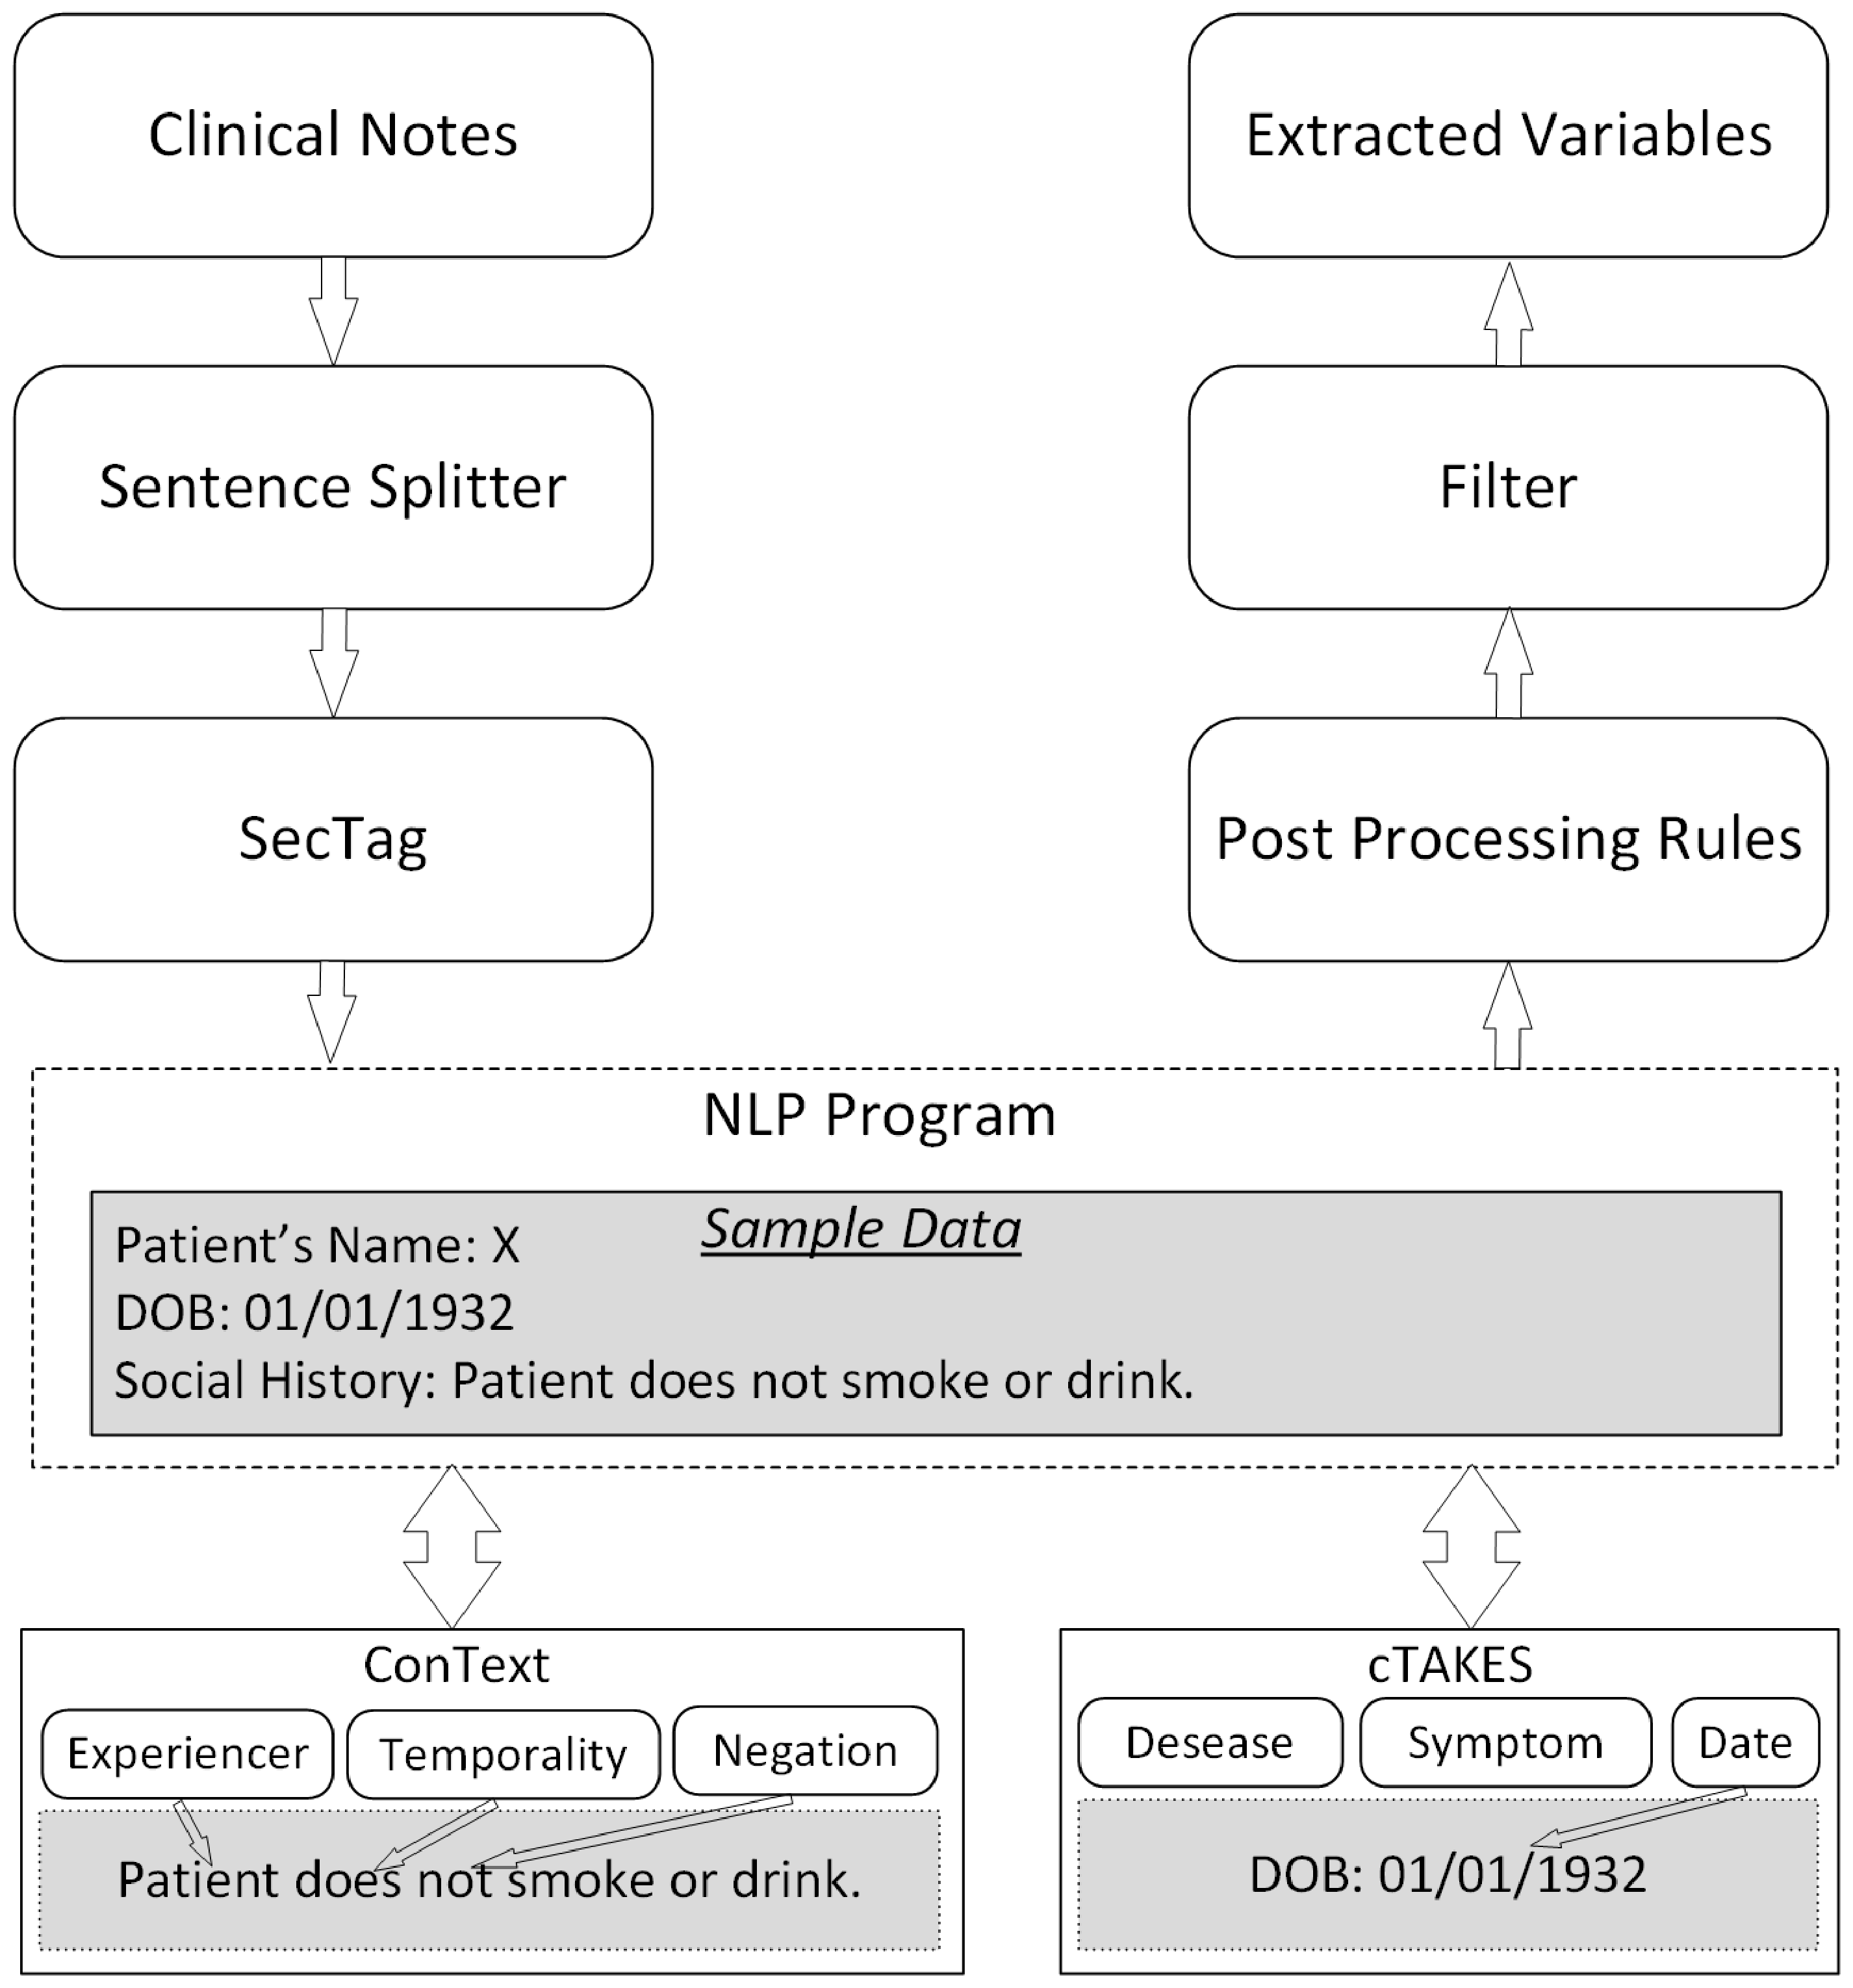
\includegraphics[width=0.5\textwidth]{figures/extraction.eps}
\caption{An architecture of the integrated system for information extraction from free-text clinical narrative used in this study.}
\label{fig:extraction}
\end{figure}

\textbf {Sentence splitter}: Sentence detection is important and necessary task for our study because we used sentence as the basic unit of variable extraction. As sentence splitting is at the core of a many NLP activities, it is provided by most NLP frameworks and libraries. We used an open source Java tools openNLP for identifying the sentence boundary. The OpenNLP sentence detector cannot identify sentence boundaries based on the contents of the sentence. However, this tools can detect that a punctuation character marks the end of a sentence or not. In this sense, a sentence is defined as the longest white space trimmed character sequence between two punctuation marks. This rule is not applicable for the first and last sentence. The first non whitespace character is assumed to be the begin of a sentence, and the last non whitespace character is assumed to be a sentence end.

\textbf {Section identification}:
Electronic health records are often divided into sections, or segments, such as ``past medical history'', ``family history'', ``assessment and plan'', etc. One can gain better understanding of clinical documents by recognition of the section in which a concept lives. For instance, both a ``past medical history'' and the ``family history'' sections can contain a list of diseases, but the context describes very different import to the patient about whom the note was written. We used SecTags for accomplishing the following three tasks: 1) excluding false positive by recognizing experiencer (patient or family member) mentioned in the family history sections; 2) determine scope of the temporal information, e.g. all events mentioned in the past medical history were historical event; 3) extract demographic information about patient from the 1st section.

\textbf {NLP program}:
As follows from Figure 1, a regular expression based NLP program was developed that utilizes the clinical Text Analysis and Knowledge Extraction System (cTAKES), which is an open source NLP and IE framework developed by the Mayo Clinic for information extraction from EHRs. This tool is comprised of several important components: sentence boundary detector, tokenizer, part-of-speech tagger, shallow parser, named entity recognizer, concept mapper, negation and status attribute detector. These components were trained on clinical text to create rich linguistic and semantic annotations of EHRs. In our study, concept mapping is used to annotate several important concepts, such as sign and symptoms, disease and disorder, lab procedure, negation and other clinical concepts.

Although most components of cTAKES have been shown to achieve good performance on a variety of NLP tasks, it has some limitations  \cite{savova2010mayo} related to certainty detection and temporal resolution. For this reason, we used ConText and semantic rules to identify temporal information. ConText is an expansion of NegEx. It relies on the same basic algorithm but applies different term lists and different windows of scope depending on the contextual feature being annotated.
 
In total, eighteen variables were extracted in this study. Since demographic variables are generally mentioned in the header or 1st section of the EHRs, we used this section for the extraction of age, sex and race. Age was determined by calculating the time period between ``date of birth'' and ``visit date or report date'', which were annotated by cTAKES. Sex and race were extracted by using simple regular expression in conjunction with a list of trigger terms such as male, female, white, african american etc. It was also confirm that the scope of the trigger term is outside the family member or relatives. We applied exactly same patterns for the extraction of ``COPD history'', ``emphysema'', ``asthma'', ``pneumonia'' and ``prior cancer''. At first, we find the triggered term or UMLS concept we are interested in. Then, we checked that the concept was not negated or fall into different experiencer such as family member. Finally, we confirmed the certainty of concept so that it was not uncertain or hypothetical such as ``suspected for pneumonia'', ``pneumonia vaccine'', etc. We also applied the semantic rules to extract ``lung cancer family history'' and ``chest x-ray in the past three years''. In addition to that, we  checked the experiencer for ``lung cancer family history'', and compared the ``visit date or report date'' with the x-ray date.

\begin{table}[h!]
\centering
\caption{Example of information extraction rules.}
\label{tab:rule}
  \begin{tabular}{|l|l|}
  \hline
    \textbf{Rule}  & \textbf{Example} \\ \hline    
    
 quit smoking \textless duration\textgreater\hspace{1mm}ago or quit smoking since \textless time\textgreater & quit smoking 30 years ago or quit smoking \\
 or quit smoking from \textless time\textgreater &  since 1960 or quit smoking from 1880 \\ \hline
  
 \textless amount\textgreater\hspace{1mm}(cigarettes\textbar pack of cigarettes) per (day\textbar week\textbar month) & 10-15 cigarettes per day or \\
 or \textless amount\textgreater\hspace{1mm}(pack\textbar pack-) year of smoking history & 30 pack year of smoking history \\ \hline
  
 (smoking\textbar smokes\textbar smoked\textbar) for \textless duration\textgreater\hspace{1mm} or & he has been smoking for 45 years or \\
 (smoking\textbar smokes\textbar smoked\textbar) (since\textbar from) \textless year\textgreater\hspace{1mm} &  he has been smoking since 1965 \\ \hline
 
  \end{tabular}
\end{table}

Smoking status is extracted using a rule based method \cite{cohen2008five, uzuner2008identifying}, which consists of two steps: hot-spot identification and post-processing rules. At first, we find the hot-spots based on keywords and sections (in many cases, smoking status was found in history and demographic sections). When a document containing one of the terms ``smok'', ``tob'', ``packs'', ``cigar'' etc. was found, a window of text up to 100 characters before and after those terms is considered as a hot-spot. Rules are then used to classify smoking status based on temporal information. After extracting the smoking status, we extracted associated information such as smoking duration, quit time and pack-year history. Several rules were employed to extract clinical variables, some of which are shown in Table~\ref{tab:rule}.

\textbf {Post processing and filter}:
To allow direct comparison between the extracted results from EHRs and PLCO results, post processing of the proposed system's output stage was required. The output of NLP program is a set of pivot text snippets such as ``two packs of cigarettes per day'', ``quit smoking in 1993'', ``smoked from the age of 18'', etc. These text fragments are then parsed to generate numeric values. Finally, the output of post-processing was filtered by keeping the latest information, for instance, a non-smoker can be a smoker after few months. To generate numeric values for statistical analysis, simple regular expression is used together with a list of terms such as ``half'', ``two'', ``one and half'', etc.

\subsection*{\textit{Statistical inference and treatment of missing values}}
Missing data frequently occur in electronic health records, which is a very common problem in data mining and statistical inference. According to Little and Rubin \cite{little2014statistical,rubin1976inference}, missing data can be categorized into three types: i) missing completely at random (MCAR)-the absence of a data element is not associated with any other value in the data set, observed or missing; ii) missing at random (MAR)-this is a less restrictive assumption than MCAR; the probability of data being missing depends only on the observed values in the data set, not on unobserved data. The implied information of missingness can be inferred from observed values; ii) not missing at random (NMAR)-the condition is opposite of MAR. The probability of data being missing depends on unobserved (missing) data. Under this circumstance, the missing information cannot be inferred from observed values. 

In order to improve the quality of research, it is important to understand the kind of missing data present in EHRs. However, missing values mechanisms are difficult to identify, because it would require the knowledge of the missing values themselves \cite{little2014statistical}. Naturally, MNAR is very difficult to be detected. This is even more complicated in case of multivariate data, outliers, inhomogeneous data or very skewed data distribution. In this paper, we explained the missingness in terms of the above mechanisms with matrix and scatter plots. Several approaches have been used to deal with missing data. The methods for coping with missing values can be grouped into three main categories \cite{little2014statistical}: inference restricted to complete data, imputation-based approaches, and likelihood-based approaches.

The simplest and most common approach to handling missing values is to omit the cases with missing values and do the analysis based only on the complete cases. Data set obtained by the result of this process can be a biased sample of complete cases because the missing of data is not a random process (i.e. data is not always MCAR). Furthermore, excluding patients with missing data will lead to a loss in statistical power. 

In imputation-based methods, the missing values are filled in and the resultant data can be analyzed as a complete data set. Imputation of missing data in the setting of MCAR will increase power but should not change the point estimates from those obtained with a complete case analysis. Therefore, it seems reasonable to perform imputations using EHR data under the assumption of MAR. Commonly imputed values are based on the value of known cases: the mean of the variable in either the whole data set or in select data subsets, or an estimated value from regression procedures on known variables. Multiple imputation methods, i.e., filling with more than one value, have been developed to avoid biasing the variances of imputed variables \cite{enders2006primer}.

There exist approaches that derive a prediction model by inferring the model's parameters from the existing data, rather than imputing data where values are missing. Likelihood-based approaches are an example of these. They developed a model by attempting to find the set of model parameters that make the observed data most likely. The resulting system parameters can then be used as the base for future inferences. The expectation maximization (EM \cite{dempster1977maximum}) algorithm is commonly used for finding maximum likelihood estimates in the face of incomplete data.

\subsection*{\textit{Evaluation methods}}
The golden standard for the evaluation of information extraction methods was created based on the EHRs collected from Henry Ford Health Systems. Each patient comprised of several EHR documents. All EHRs were manually investigated by domain expert to find the values of target variables for each patient. Then, we compared the values of extracted categorical and non-categorical (continuous) variables with gold standard to evaluate the accuracy of IE. 

\section*{Results}
We present the results and outcomes of our study regarding the performance of information extraction from EHRs and statistical significance between EHR extraction and PLCO survey response. \\

%We begin presentation of our experimental results with an analysis of the quality of extraction against PLCO survey re-sponses as well as the missing patterns in extracted and survey variables, and conclude with comparing the outcomes of lung cancer risk factors identification and prediction models on both datasets. Table 2 shows the distribution of data for both PLCO and EHRs.\\

\begin{table}[h]
\centering
\caption{Performance of information extraction from electronic medical record prepared with 1000 samples from the entire population.}
\label{tab:result1}
  \begin{tabular}{|l|l|l|l|l|l|}
  \hline
    \multirow{2}{*}{\textbf{Variables}}  & \multicolumn{2}{c|}{\textbf{Retrieved}}  & \multirow{2}{*}{\textbf{Not Retrieved (\%)}} & \multirow{2}{*}{\textbf{Accuracy}} \\ \cline{2-3}
    
 & \textbf{Correct} & \textbf{Wrong (\%)}  &  &  \\ \hline    
    
 Age & 998 & 2 (0.20\%) & 0 (0\%) & 0.998\\ \hline
 Sex & 975 & 7 (0.70\%) & 0 (0\%) & 0.975\\ \hline 
 Race & 999 & 1 (0.01\%) & 0 (0\%) & 0.999\\ \hline
 Lung cancer family history & 996 & 4 (0.40\%) & 0 (0\%) &  0.996\\ \hline
 COPD history & 987 & 13 (1.30\%) & 0 (0\%) & 0.987\\ \hline
 Chest x-ray in last 3 years & 1000 & 0 (0\%) & 0 (0\%)  & 1.000\\ \hline
 Emphysema & 994 & 6 (.60\%) & 0 (0\%) &  0.994\\ \hline
 Asthma & 995 & 5 (0.50\%) & 0 (0\%) &  0.995\\ \hline
 Prior cancer & 962 & 38 (3.80\%) & 0 (0\%) &  0.962\\ \hline
 Pneumonia & 982 & 18 (1.80\%) & 0 (0\%) & 0.982\\ \hline
 Hay fever & 999 & 1 (0.10\%) & 0 (0\%) &  0.999\\ \hline
 Smoking status & 912 & 88 (8.80\%) & 0 (0\%)  & 0.912\\ \hline
 Smoker status & 490 & 18 (3.53\%) & 2 (0.40\%) &  0.961\\ \hline
 Age at start smoking & 10 & 1 (5.26\%) & 8 (42.11\%) & 0.526\\ \hline
 Smoking amount (\# cigarettes per day) & 277 & 24 (7.62\%) & 14 (4.44\%) & 0.879\\ \hline
 Smoking duration & 191 & 16 (6.58\%) & 36 (14.81\%) & 0.786\\ \hline
 Quit time of former smoker & 241 & 6 (2.31\%) & 13 (5.00\%) & 0.927\\ \hline
 Pack-years smoked & 212 & 18 (6.84\%) & 33 (12.55\%) & 0.806\\ \hline 
 
  \end{tabular}
\end{table}

%\begin{table}[h]
%\centering
%\caption{Performance of information extraction from electronic medical record prepared with 1000 samples from the entire population.}
%\label{tab:result1}
%  \begin{tabular}{|l|l|l|l|l|l|}
%  \hline
%    \multirow{2}{*}{\textbf{Variables}}  & \multicolumn{2}{c|}{\textbf{Retrieved}}  & \multirow{2}{*}{\textbf{Not Retrieved}}   & \textbf{Missing in}  & \multirow{2}{*}{\textbf{Accuracy}} \\ \cline{2-3}
%    
% & \textbf{Correct} & \textbf{Wrong}  & & \textbf{EHR} &  \\ \hline    
%    
% Age & 998 & 2 & 0 & 0 & 0.998\\ \hline
% Sex & 975 & 7 & 0 & 18 & 0.975\\ \hline 
% Race & 977 & 1 & 0 & 22 & 0.977\\ \hline
% Lung cancer family history & 996 & 4 & 0 & 0 & 0.996\\ \hline
% COPD history & 987 & 13 & 0 & 0 & 0.987\\ \hline
% Chest x-ray in last 3 years & 1000 & 0 & 0 & 0 & 1.000\\ \hline
% Emphysema & 994 & 6 & 0 & 0 & 0.994\\ \hline
% Asthma & 995 & 5 & 0 & 0 & 0.995\\ \hline
% Prior cancer & 962 & 38 & 0 & 0 & 0.962\\ \hline
% Pneumonia & 982 & 18 & 0 & 0 & 0.982\\ \hline
% Hay fever & 999 & 1 & 0 & 0 & 0.999\\ \hline
% Smoking status & 912 & 88 & 0 & 0 & 0.912\\ \hline
% Smoker status & 490 & 18 & 2 & 490 & 0.980\\ \hline
% Smoking start age & 10 & 1 & 8 & 981 & 0.991\\ \hline
% Smoking amount (\# cigarettes per day) & 277 & 24 & 14 & 685 & 0.962\\ \hline
% Smoking duration & 191 & 16 & 36 & 757 & 0.948\\ \hline
% Quit time of former smoker & 241 & 6 & 13 & 740 & 0.981\\ \hline
% Pack-years smoked & 212 & 18 & 33 & 737 & 0.949\\ \hline 
% 
%  \end{tabular}
%\end{table}

\subsection*{\textit{Performance of information extraction from EHRs}}
Table~\ref{tab:result1} shows the performance of our system evaluated with the gold standard on the 1000 patients randomly selected from the 11,968 patients. Performance was the best with chest x-ray identification (100\%) and was good (approximately 99\% accuracy) for age, race, lung cancer family history, emphysema, asthma and hey fever. Results were above 90\% accurate for sex, COPD history, prior cancer, pneumonia, smoking status and smoker status, except smoking duration, smoking amount and pack-year smoked with 78.6\%, 87.9\% and 80.6\% accuracy, respectively. Our system performed worst when identifying ``age at start smoking''. However, the system unable to retrieved 0.40\%, 42.11\%, 4.44\%, 14.81\%, 5\% and 12.55\% information regarding the variables smoker status, age at start smoking, smoking amount, smoking duration, quit time of former smoker and pack-year smoked. The NLP program provides 8.80\%, 0.50\%, 3.8\%, 1.8\%, , 7.62\%, 3.53\% and 6.84\% incorrect result when identifying  smoking status, asthma, prior cancer, pneumonia, smoking amount, smoker status and pack-year smoked, respectively. \\

\begin{table}[h!]
\centering
\caption{Results of information extraction from electronic health record compared with PLCO trial on the 1000 patients subset.}
\label{tab:result2}
  \begin{tabular}{|l|l|l|l|l|l|}
  \hline
    \textbf{Variables}  & \textbf{Agreed by }  & \textbf{Correct in}   & \textbf{Correct in}  & \textbf{Information Missing} \\
      & \textbf{EHR and PLCO}  & \textbf{EHR}   & \textbf{PLCO}  & \textbf{from EHR} \\ \hline    
    
 Age & 992 (99.2\%) & 6 (0.60\%) & 2 (0.20\%) & 0 (0\%) \\ \hline
 Sex & 964 (96.4\%) & 11 (1.1\%) & 7 (0.70\%) & 18 (1.8\%) \\ \hline 
 Race & 949 (94.9\%) & 28 (2.8\%) & 1 (0.10\%) & 22 (2.2\%) \\ \hline
 Lung cancer family history & 906 (90.6\%) & 25 (2.5\%) & 4 (0.40\%) & 65 (6.5\%) \\ \hline
 COPD history & 873 (87.3\%) & 68 (6.8\%) & 13 (1.3\%) & 46 (4.6\%) \\ \hline
 Chest x-ray in last 3 years & 546 (54.6\%) & 19 (1.9\%) & 26 (2.6\%) & 409 (40.9\%) \\ \hline
 Emphysema & 933 (93.3\%) & 29 (2.9\%) & 6 (0.6\%) & 32 (3.2\%) \\ \hline
 Asthma & 86 (8.6\%) & 0 (0\%) & 5 (0.50\%) & 909 (90.9\%) \\ \hline
 Prior cancer & 677 (67.7\%) & 0 (0\%) & 38 (3.8\%) & 285 (28.5\%) \\ \hline
 Pneumonia & 106 (10.6\%) & 0 (0\%) & 18 (1.8\%) & 876 (87.6\%) \\ \hline
 Hay fever & 13 (1.3\%) & 0 (0\%) & 1 (0.1\%) & 986 (98.6\%) \\ \hline
 Smoking status & 611 (61.1\%) & 99 (9.9\%) & 88 (8.8\%) & 202 (20.2\%) \\ \hline
 Smoker status & 488 (48.8\%) & 2 (0.20\%) & 18 (1.8\%) & 492 (49.2\%) \\ \hline
 Age at start smoking & 10 (1\%) & 0 (0\%) & 9 (0.90\%) & 981 (98.1\%) \\ \hline
 Smoking amount (\# cigarettes per day) & 277 (27.7\%) & 0 (0\%) & 38 (3.8\%) & 685 (68.5\%) \\ \hline
 Smoking duration & 191 (19.10\%) & 0 (0\%) & 52 (5.2\%) & 757 (75.7\%) \\ \hline
 Quit time of former smoker & 241 (24.1\%) & 0 (0\%) & 19 (1.9\%) & 740 (74\%) \\ \hline
 Pack-years smoked & 212 (21.2\%) & 0 (0\%) & 51 (5.1\%) & 737 (73.7\%) \\ \hline 
 
  \end{tabular}
\end{table}

\begin{figure}[h!]
\centering
\includegraphics[width=1.0\textwidth]{figures/matrixplot.eps}
\caption{Matrix plots demonstrate the MAR situation among variables.}
\label{fig:matrixplot}
\end{figure}

\subsection*{\textit{Comparing the results between EHR extraction and PLCO survey response}}
To compare the results from the proposed system directly with PLCO survey response, the same 1000 cases were compared. Table~\ref{tab:result2} presents the EHR results compared with PLCO clinical trial response. This results revealed some interesting findings.

First, highest agreement of results by both EHR and PLCO is observed in age value, achieved 99.2\% agreement against gold standard. The main reason is that ``date of birth'' is well formatted and structured across all reports. However, lowest agreement (1\%) is examined for ``age at start smoking''. The common reason might be the ambiguity between patient age and smoking age or difficulties to create an extraction system for identifying ``age at start smoking''. The values extracted from EHRs were agreed well with PLCO responses for the variables ``sex'',``race'',``lung cancer family history'',``COPD history'' and ``emphysema'' in 96.4\%, 94.9\%,90.6\%, 87.3\% and 93.3\% cases, respectively. On the other hand, ``chest x-ray in last 3 years'', ``prior cancer'', ``smoking status'' and ``smoker status'' were moderately agreed by PLCO and EHR extraction.    

Second, we observed a certain percentage of disagreement between PLCO and EHR results. Compared to gold standard, EHR results are correct in some cases while PLCO are correct in other cases. The highest disagreement was noticed in ``smoking status'' where EHR results (9.9\%) have higher accuracy compared to PLCO results (8.8\%). Error occurred most frequently in EHR results for many variables due to the assumption that either the value is missing or has a default value. For example, we assigned the default value ``non-smoker'' to the smoking status, when system fails to find any information related to smoking status. Because of this, ``asthma'', ``prior cancer'', ``pneumonia'', ``hay fever'', ``age at start smoking'', ``smoking amount'',``smoking duration'', ``quit time of former smoker'' and ``pack-year smoked'' were only correct in PLCO when disagreed with EHR results. Certain variables such as ``age'', ``sex'', ``race'', ``lung cancer family history'' and ``COPD history'' provided higher percentage of correct values in EHRs compared to PLCO response. Contrarily, PLCO results provided higher percentage of accurate results for the variables ``chest x-ray in last 3 years'' and ``smoker status''. 

Finally, highest number of missing values is observed in ``hay fever'', which displayed 98.6\% missing values in EHRs. However, no value is missing for the variable age. Although we observed a significant number of missing values in smoking related variables, around 50\%-70\% values are missing due to the non-smokers or former smokers. Therefore, there are few percentage of actual missing values for the variables ``smoker status'', ``age at start smoking'', ``smoking amount'', ``smoking duration'', ``quit time of former smoker'' and ``pack-year smoked''. 

\subsection*{\textit{Missing pattern analysis}}
We utilized all patients participated in PLCO clinical trials for the analysis of missing values. Figure~\ref{fig:matrixplot} shows the MAR situation among variables where the sorting was done by quit time, age and status, respectively. It can be seen that the higher the quit time, the more missing values in the variables smoking amount and pack-year smoked. On the other hand, missing values increase with the decrements of quit time. It was also shown that more missing values were observed for sex and race when age values are decreasing. Furthermore, they were more likely missing from EHR when smoking status is unavailable.   

\begin{figure}[h!]
\centering
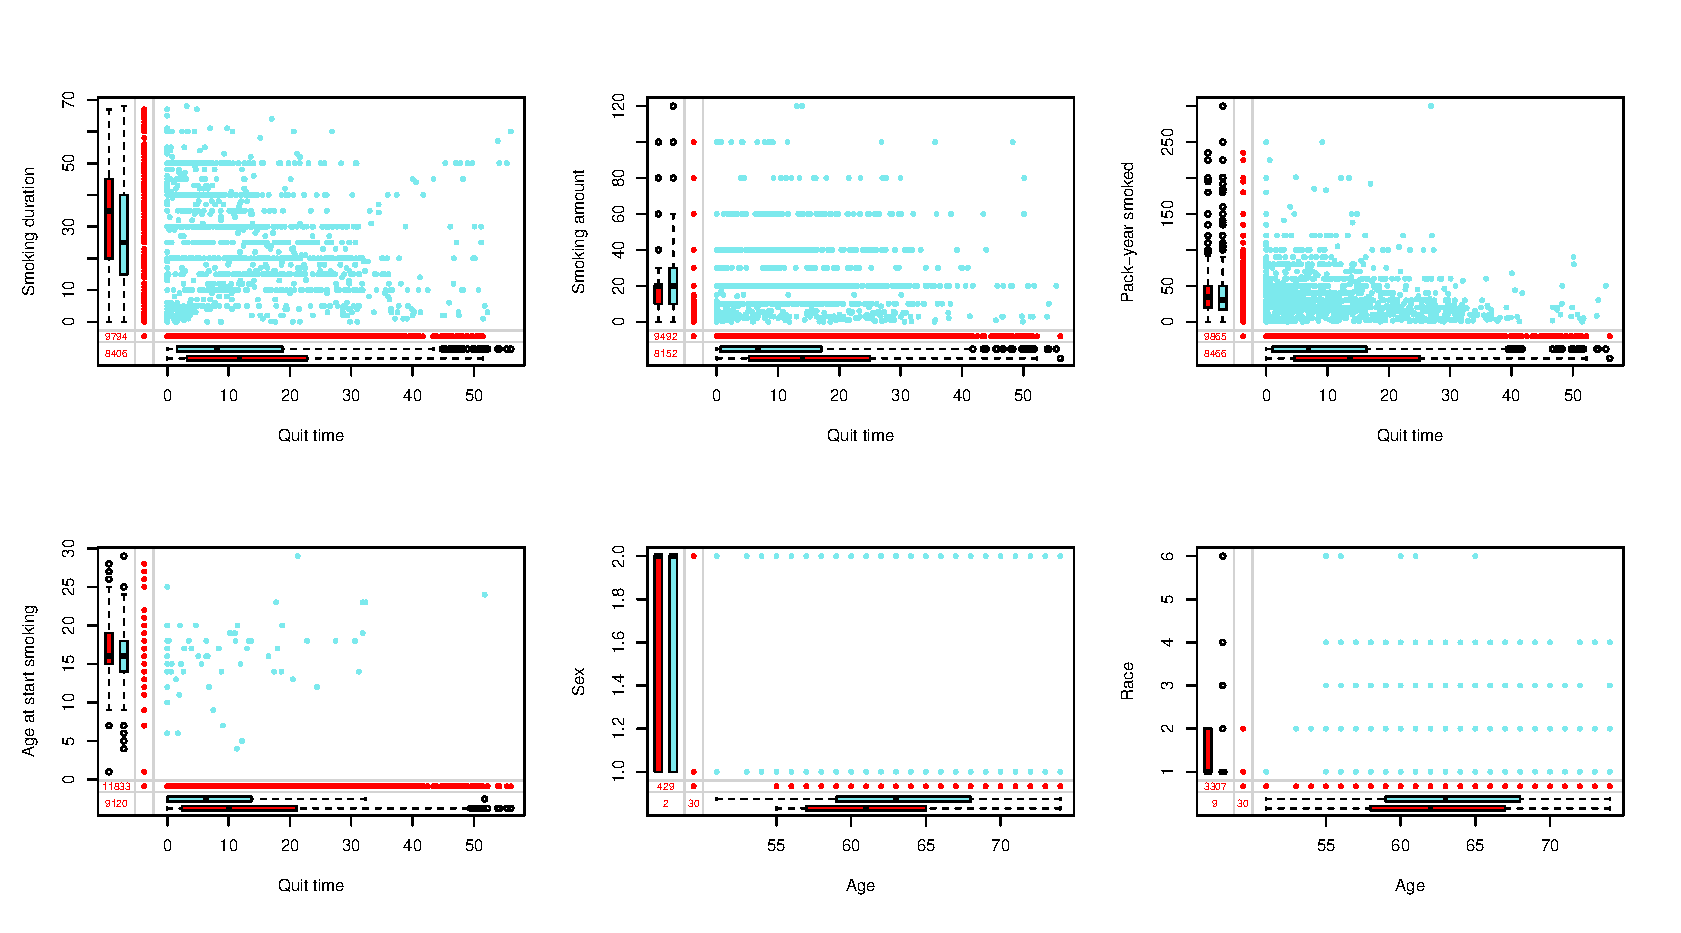
\includegraphics[width=1.0\textwidth]{figures/marginplot.eps}
\caption{Scatter plots illustrate the MAR situation between variables.}
\label{fig:marginplot}
\end{figure}

The MAR relations were observed more clearly in Figure~\ref{fig:marginplot}. Along the horizontal axis, the red boxplot is for those values of x (i.e. quit time, age) where no values for y (i.e. pack-year smoked, smoking amount) are available, and the blue boxplot for x values where also information for y is available. A comparison of the two boxplots can indicate the missing data mechanism. For example, the quit time for former smokers that provide no information for smoking amount seems to be higher than that where information is available. 

\section*{Discussion}
In this study, we investigated errors of extracting information from EHRs to characterize the reasons for disagreement between extracted values and report values. This information have significant value in establishing priorities for the development of an Information Extraction System in Bio-medical domain as well as conducting clinical trials. 

The results suggest that automated extraction of clinical information may be more valid for some variables, and less valid for others. In spite of disagreements between information in the reports, automatic information extraction could still be beneficial for quick access to information, depending on the error threshold a user can withstand. For example, EHR data provide nearly the human accuracy for variables such as age, sex, race, lung cancer family history, COPD history and emphysema. Furthermore, less than 1\% disagreement were observed only with PLCO responses, so the information extracted could still be extremely useful.

Numerous errors were observed, where quantitative information extraction errors were the most prevalent among all variables. Several formats were observed in various report with different sentence structures. Furthermore, spelling error, ungrammatical structure, abbreviation and acronym create this extraction process more difficult. For instance, quit time of former smoker needs to be extracted from the clause ``q age 20''. We can calculate it with (current age - 20) by identifying q and age as ``quit time'' and ``age at quited from smoking''.  

For medical condition extraction, the most common failure was due to errors in section boundary and ambiguous pronoun. If the section of the current sentence is not identified correctly, we will not be able to extract the medical condition such as lung cancer family history, COPD history, pneumonia, asthma, etc. Many of the false positive were due to ambiguous pronoun that may refer family member instead of patient.

A  few data inconsistencies were observed in some of the variables such as sex and race. In order to determine the status of sex, we needed to determine the presence or absence of UMLS concepts that represent sex, such as ``male'', ``woman'', ``gentleman'', ``lady'', etc. However, we observed information mismatch between or within the same EHR data source.

In order to choose a proper imputation method one must be aware of the missing data mechanism(s). The quality of the imputed values depends on the imputation itself and on the imputation method used. In this study, matrix and scatter plots were used to determine the missing data mechanism(s) among variables. We demonstrate that there were MAR relation between quit time and smoking amount, quit time and smoking duration, quit time and pack-year smoked, age and sex, and age and race.

\section*{Conclusion}
In this paper, we compared result of the integrated systems with PLCO clinical trials and observed that the performance of the systems rivaled the clinical trial, when clinical information appears in electronic health records. However, clinical trial is necessary for certain variables such as ``age of start smoking'', ``education'', ``occupation'', etc. The proposed system consists of several state-of-the-art NLP systems to identify patients information from electronic health records. Experimental result shows 91.2\% to 100\% accuracy in retrieved variables. This study also provides an analysis of some of the
difficulties that could be encountered in extraction of information from free-text clinical reports to automatically extract variables. Each of the
variables had a different profile of errors, suggesting that some variables may be ``better targets'' for information extraction and auto-annotation than others. Finally, we addressed data missingness issue and reviewed different mechanisms through which data may be missing. The absence of data elements is the consequence of physician decisions and reflects aspects of the patient's condition. As the absence of data is usually considered a hindrance to accurate computer-based diagnosis, we need proper treatment of missing data. In this paper, we present missing patterns with matrix and scatter plots, and suggest various ways of dealing with missing values including ``multiple imputation'', ``use of means'', etc.  

\section*{Acknowledgments}
We would like to thank the technical staff at Henry Ford Health Systems and Textual Data Analytics Laboratory at Wayne State University for their help with collecting and transforming binary data into free text EHR used for experiments reported in this paper. 

\bibliographystyle{vancouver}
\bibliography{references}

\end{document}